%**************************************************************
% Capitolo 2 - PERCHÉ - Scelta dello stage e rapporto con l'azienda
%**************************************************************
\chapter{Scelta dello stage e rapporto con l'azienda}
%TODO: introduzione capitolo

\section{Lo stage per l'azienda}

   \subsection{Necessità dell'azienda}
   \nomeAzienda{} sta sviluppando un sistema di videoconferenza per assistenza remota da applicare ai lavori specialistici e all'interno di aziende manifatturiere. Il sistema è pensato per aiutare un lavoratore inesperto, in situazioni difficili, facendolo guidare da una persona con le conoscenze adeguate a svolgere tali mansioni. Per rendere l'esperienza pratica funzionale, l'azienda ha pensato di utilizzare dei visori per la realtà aumentata, concentrandosi particolarmente sui Google Glass. L'utente esperto dovrà essere in grado di vedere in tempo reale quello che l'altro vede, tramite una videocamera integrata negli occhiali, e di mostrargli dati ed indicazioni su quello che deve fare, tramite il display integrato. Per realizzare tale progetto, \nomeAzienda{} necessita di un'intera piattaforma di streaming, che sta realizzando a componenti nel corso del tempo.
   \begin{figure}[H]
      \begin{center}
         
\includegraphics[width=16.5cm,keepaspectratio]{immagini/erastreaming-schema}
      \end{center}
      \caption{Schema generale del funzionamento della piattaforma di streaming}
   \end{figure}
   Il sistema che l'azienda vuole costruire è composto da tre elementi fondamentali, il client dell'utente sul campo, il sistema di relay e il client dell'utente esperto. Il primo è realizzato con uno smartphone Android e un paio di Google Glass; permetterà di registrare audio e video, inviati al sistema di relay tramite la rete del telefono, e di ricevere audio, video o messaggi di testo, inviati dal secondo client. Il client dell'utente esperto deve permettere di visualizzare e ascoltare i dati ricevuti e di poter rispondere con dati simili, per indicare al primo utente le azioni da compiere. Infine, il sistema di relay è composta da due elementi, un cluster di server di relay e un server amministratore; il primo è quello che si occupa del reinvio dei messaggi e della continuità della trasmissione tra i client connessi, mentre il secondo è adibito alla gestione dei canali, dell'autenticazione degli utenti e del bilanciamento del carico tra i nodi di relay.
   \\
   \nomeAzienda{} ha già realizzato un prototipo di client Android del servizio e, dopo test di trasmissione interni al dispositivo, si sta preparando per il passaggio alla comunicazione tra due dispositivi connessi ad una rete locale. Successivamente l'azienda provvederà a creare un sistema di amministrazione sfruttando Firebase e il suo servizio di autenticazione sicura.
   \begin{figure}[H]
      \begin{center}
         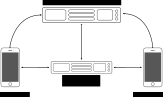
\includegraphics[width=12cm,keepaspectratio]{immagini/erastreaming-schema-attuale}
      \end{center}
      \caption{Schema delle componenti in fase di sviluppo}
   \end{figure}
   L'Obiettivo dello stage è quello di sviluppare il software del server di relay, necessario per far comunicare i due client. Il server deve permettere ai due dispositivi di inviarsi messaggi di qualsiasi tipo, senza che uno conosca l'indirizzo di rete dell'altro, e di gestire i canali e gli utenti tramite un API amministratore.
   
   \subsection{Risultati degli stage precedenti e seguito degli stagisti nell'azienda}
   \nomeAzienda{} ha deciso anche quest'anno di partecipare all'evento ``StageIt'', organizzato da Confindustria Padova in collaborazione con l'Università degli Studi di Padova, e di proporre agli studenti un tirocinio interno all'azienda. L'impresa è alla ricerca di neolaureati per arricchire il proprio team di sviluppatori, dato il recente aumento di clienti e la conseguente espansione.
   \nomeAzienda{} è, in particolare, interessata a studenti che sono appassionati di nuove tecnologie e che hanno interesse a imparare nuove tecniche e a farne conoscere di nuove all'azienda stessa.
   L'impresa ha già organizzato tirocini con altri studenti negli anni precedenti, ottenuto risultati soddisfacenti, tanto che molti degli ex stagisti sono stati assunti dall'azienda.

\section{Rapporto con il mio stage e con l'azienda}
   \subsection{Ambiti di interesse}
   Al momento della ricerca di uno stage ho prestato particolare attenzione alle aziende che proponevano un percorso legato ai miei interessi di studio. In particolare cercavo tirocini il cui argomento fosse compreso tra i seguenti:
   \begin{itemize}
      \item{Sicurezza;}
      \item{Sistemi ad alta concorrenza;}
      \item{Dispositivi IoT;}
      \item{Sistemi virtualizzati;}
      \item{Servizi cloud;}
      \item{DevOps;}
      \item{Sistemi multimediali.}
   \end{itemize}

   \subsection{Proposte di stage ricevute}
   Nei giorni immediatamente seguenti all'evento StageIt sono stato contattato da alcune aziende presenti delle quali ho selezionato le proposte che più mi parevano interessanti.
   \\
   Uno dei progetti proposti consisteva in un sistema di controllo di risorse e consumi di sistemi virtualizzati tramite \gls{Docker}: il software doveva fornire una chiara visione dello stato di ciascun servizio e riportare eventuali anomalie. Lo stage mi avrebbe permesso di conoscere meglio l'utilizzo di Docker, specialmente in un contesto DevOps, e di imparare nuove tecnologie di gestione di gruppi di contenitori, in particolare Kubernetes; fondamentali in un contesto di continuous deployment e continuous release. Le conoscenze che mi avrebbe fornito questo tirocinio erano di mio grande interesse, ma, sfortunatamente, non sono stato scelto, tra i possibili candidati.
   \\
   Un altro stage riguardava la realizzazione di un software in grado di unificare la grande mole di dati dell'azienda, sparsa tra diversi sistemi aziendali legacy e i \gls{CMS} dei loro clienti. Il prodotto avrebbe dovuto raccogliere i dati, salvarli in un formato comune, facilmente accessibile, e aggiornare i sistemi in caso di modifiche. L'utilità di un software del genere è molto elevata per un'azienda, ma il prodotto in sé consiste in un certo numero di adattatori per ciascuna delle fonti di dati, e non mi avrebbe fornito particolari conoscenze aggiuntive, rispetto a quelle che già possedevo.
   \\
   Un altro progetto proposto, invece, prevedeva la realizzazione di un sistema per la gestione delle traduzioni dei testi di un catalogo prodotti, consentendo visualizzazione, modifica e la ricerca di testi ripetuti tramite Elasticsearch, per l'ottimizzazione delle spese di traduzione. Elasticsearch è un motore di analisi del testo il cui utilizzo si sta diffondendo molto in fretta, ma lo stage non comprendeva lo studio del suo funzionamento. Il prodotto avrebbe anche dovuto generare una serie di informazioni, come un preventivo dei costi di traduzione e una lista di frequenza di certe espressioni.
   \\
   Un ulteriore tirocinio prevedeva un progetto sperimentale per lo spostamento di un software di rendering \gls{CAD} per \gls{TAC} da un sistema locale a uno client-server, con elaborazione dei dati su server virtualizzati. Il video elaborato sarebbe poi stato servito a un \gls{thin client}; alleggerendolo del carico di computazione del render. Il progetto comportava la scomposizione del software proprietario dell'azienda, lo studio di una soluzione di virtualizzazione e l'integrazione con una libreria per la trasmissione dei dati. Sebbene lo stage proposto toccasse molti e vari ambiti, si sarebbe concentrato solo in una parte del progetto, prevedendo la continuazione da parte dello studente dopo la laurea. Considerata la mia scelta di continuare i miei studi, non ho potuto accettare la proposta dell'azienda.

   \subsection{Scelta dello stage}
   %TODO: espandere sezione
   Al momento della scelta di quale stage accettare, tra quelli proposti, ho preferito optare per quello che proponeva argomenti per me più nuovi e meno conosciuti, che producesse, quindi, il migliore valore aggiunto per mie competenze.
   Ho scelto il progetto di \nomeAzienda{} perché ho trovato il campo di cui si occupa interessante e le mie conoscenze sull'argomento erano solo marginali. Inoltre una più approfondita conoscenza di sistemi ad alta concorrenza, come può essere un servizio di streaming, è applicabile a molti altri campi, come sistemi cloud distribuiti e dispositivi IoT.

   \subsection{Scelta dell'azienda}
   Durante la scelta dello stage ho considerato marginale l'aspetto del futuro in azienda, dato che la mia scelta di continuare a studiare per la laurea magistrale è incompatibile con un lavoro a tempo pieno. Il mio interesse più grande era quello di poter collaborare con persone più esperte di me per imparare cose nuove; per questo motivo mi sono accertato che durante il tirocinio avrei potuto interagire con molte figure dell'azienda che si occupano di sviluppo.
   \\
   Un altro importante fattore che ho deciso di ignorare è stata la distanza dell'azienda dalla mia residenza: ho preferito dare più importanza all'esperienza dello stage in sé rispetto alla comodità di spostamento.

\section{Obiettivi del progetto di tirocinio}
All'inizio del progetto di tirocinio sono stati definiti gli obiettivi, distinti poi in obbligatori e desiderabili, e i vincoli tecnologici ai quali ho dovuto attenermi. Ne segue una lista dei fondamentali.

   \subsection{Obiettivi obbligatori}
   \begin{itemize}
      \item{Studio dei formati video e dei protocolli di rete per le trasmissioni video in real-time e on-demand;}
      \item{Studio dell'architettura di rete di un servizio di streaming;}
      \item{Sviluppo di un applicativo server per il relay di messaggi tra i suoi client.}
   \end{itemize}

   \subsection{Obiettivi desiderabili}
   \begin{itemize}
      \item{Studio delle problematiche della trasmissione di dati in mobilità;}
      \item{Sistema di autenticazione dei client e organizzazione a canali delle trasmissioni;}
      \item{Studio di possibili utilizzi della tecnologia Blockchain nel campo dello streaming.}
   \end{itemize}

   \subsection{Vincoli tecnologici}
   Mi è stato richiesto di utilizzare Java come linguaggio di programmazione, per consentire una più veloce integrazione con il client Android. Inoltre, data la struttura a servizi della piattaforma, ho dovuto utilizzare un server Java come base del prodotto.

\section{Pianificazione del lavoro}
La pianificazione del progetto è stata eseguita in accordo con il tutor interno. Nella prima settimana ho avuto modo di studiare gli strumenti, i formati e i protocolli necessari alle funzioni della piattaforma, stilando una relazione sullo stato dell'arte. Ho, poi, proseguito con l'analisi delle funzionalità richieste e la definizione di requisiti e casi d'uso. Ho impiegato la terza settimana nella progettazione del servizio e della componente server, per poi procedere le due settimane successive alla sua realizzazione. Per garantire una buona qualità del codice, ho dedicato una settimana alla validazione, ai beta test e alla riformattazione. L'ultima settimana ho ultimato la documentazione del progetto e dei risultati ottenuti.
\begin{figure}[H]
   \begin{center}
      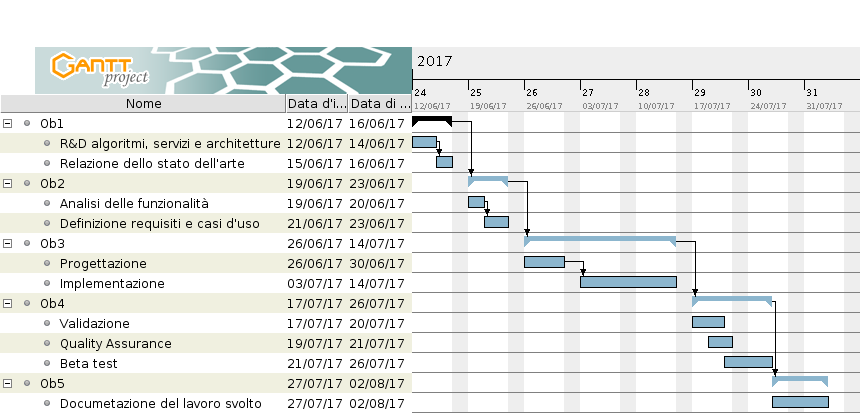
\includegraphics[height=8cm,width=15cm,keepaspectratio]{immagini/pianificazione-gantt}
      \caption{Diagramma di Gantt della pianificazione}
   \end{center}
\end{figure}

   \subsection{Strumenti utilizzati}
   Per ottenere buoni risultati durante la pianificazione \nomeAzienda{} utilizza GanttProject\footnote{Sito web del progetto GanttProject: \href{http://www.ganttproject.biz/}{www.ganttproject.biz}}, un software open-source per la realizzazione di diagrammi di \gls{Gantt} e \gls{PERT}. Il programma permette di costruire diagrammi con estrema facilità, gestendo scadenze, risorse, personale e dipendenze; inoltre permette di esportare il risultato in HTML o in formato PNG.\
